\documentclass[swedish,11pt]{article}
\usepackage[english]{babel}
\usepackage[utf8x]{inputenc}
\usepackage{times}
\usepackage[T1]{fontenc}
\usepackage{tikz}
\usetikzlibrary{arrows,snakes,backgrounds,shapes}
\usepackage{hyperref}
\textwidth=16cm
\textheight=23cm
\oddsidemargin=-0.1cm
\evensidemargin=-0.1cm
\topmargin=-2cm

\title{openRGD}
\author{Anders Ardö\\Anders.Ardo@gmail.com}
%\institute{}

\begin{document}
\maketitle

\section{Inledning}
openRGD är implementerat huvudsakligen i Python och använder
bl.a. de färdiga programbiblioteken bottle (http://bottlepy.org/docs/dev/index.html) webframework,
Beaker (https://beaker.readthedocs.org/en/latest/)
sessionshantering, bottle-cork (http://cork.firelet.net/)
autentisering och rättigheter, 
cherryPy (http://www.cherrypy.org/) webserver, libsvm
(http://www.csie.ntu.edu.tw/~cjlin/libsvm/) klassifikation, och PyLucene
(http://lucene.apache.org/pylucene/) fritextdatabas.

\section{Översikt, arbetsflöde}
\begin{figure}[htb]
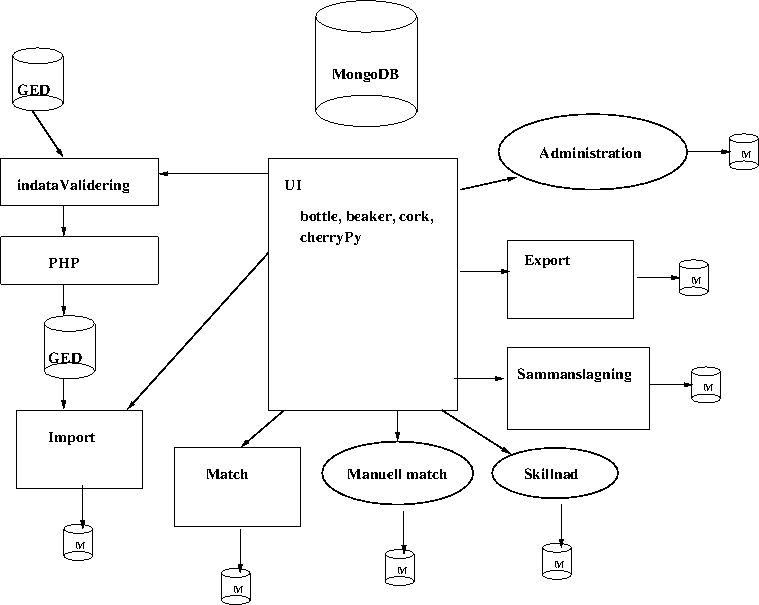
\includegraphics[width=\textwidth,height=11cm]{openRGD}
\end{figure}

Systemet består av (UI-numreringen hänvisar till sidan ``Startsida -
arbetsflöde'' i Web-gränssnittet):
\begin{itemize}
\item Web-gränssnitt - \verb+UI.py+  se http://rgd.eit.lth.se:8085 och avsnitt \ref{UI} nedan
\item Indatavalidering av Gedcom-fil - \verb+indataValidering.py+
  (UI 1-2)\\
huvudsakligen en wrapper som anropar ett antal PHP-program som
Carl-Johan Gustafsson har skrivit.
\item Import av Gedcom till databas - \verb+importGedcom.py+ (UI 3) - se
  avsnitt \ref{import} nedan
\item Maskinell matchning av två databaser - \verb+match.py+ (UI 4) - se
  avsnitt \ref{match} nedan
\item Manuell matchning/korrigering - intern funktion i
  Web-gränssnittet (UI 5)
\item Visa skillnader - intern funktion i
  Web-gränssnittet (UI 6)
\item Sammanslagning av två databaser - \verb+merge.py+ (UI 7) - se
  avsnitt \ref{merge} nedan
\item Export av en databas i Gedcom-format - \verb+exportGedcom.py+
  (UI 8) - se avsnitt \ref{export} nedan
\end{itemize}

Dessutom finns ett antal globala variabler och rutiner i filerna
\begin{itemize}
\item \verb+common.py+ globala definitioner och variabler, mongodb-klienter
\item \verb+graphUtils.py+ används i Web-gränssnitt 
\item \verb+importUtil.py+ används vid import av Gedcom-fil
\item \verb+luceneUtils.py+ används för hantering av Lucene-databaser
\item \verb+matchtext.py+ används vid matchning för att ta fram texter
  för indexering i Lucene
\item \verb+matchUtils.py+ används vid matchning
\item \verb+mergeUtils.py+ används vid sammanslagning
\item \verb+SVMfeatures.py+ används vid matchning
\item \verb+uiUtils.py+ används i Web-gränssnitt 
\item \verb+utils.py+ används i Web-gränssnitt 
\item \verb+workFlow.py+ används i Web-gränssnitt 
\end{itemize}

\section{Databasmodell}
I openRGD används mongodb (http://www.mongodb.org/) som hanterar databaser och collections (som
motsvarar tabeller i relationsdatabaser). Mongodb är en flexibel,
högprestanda noSQL dokumentdatabas. Collections består av dokument med
ett flexibelt schema som inte kräver en fix dokumentstruktur.

Ett dokument består av flera 'namn/nyckel - värde' par inom
\verb+{ }+. Namn/nyckel är bara ett namn eller nyckel som gör det
möjligt att komma åt värdet.
Ett värde kan vara data, en lista \verb+[ ]+ eller en nästlad
'namn/nyckel - värde' struktur \verb+{ }+. En lista kan innehålla
värden eller nästlade listor/'namn/nyckel - värde' strukturer. Ett enkelt exempel (men kanske
inte användbart) på hur en familj (med man, hustru och 2 barn) kan representeras i ett dokument:
\begin{verbatim}
{
  "man": {
    'namn': 'Anders Oskarsson',
    'ålder': 47
  }
  'hustru': {
    'namn': 'Kajsa Nilsson',
  }
  'barn': [
            { 'namn': 'Hans'},
            { 
              'namn': 'Else',
              'adopterad': 'JA'
            }
          ]
}              
\end{verbatim}

En databas per bidrag och en databas för RGD. Databasens namn består
av två delar - först openRGD användaren och sedan namnet på den
uppladdade Gedcom-filen sammanbundna med '\_'. T.ex. innehåller
databasen \verb+anders_demoged+ data från filen \verb+demoged.GED+ och
är skapad av användaren \verb+anders+.

Alla databaser har collections: \verb+persons, families, originalData+. Dessutom
används 2-3 temporära collections under matchningen:
\verb+matches, fam_matches, flags+. Namnen på dessa collections anger
också vilken databas som är matchad. T.ex. databasen
\verb+kalle_testp1+ kan ha collections \verb+matches_kalle_testp2+ och
\verb+fam_matches_kalle_testp2+ som innehåller resultatet från matchningen av databasen
\verb+kalle_testp1+ mot databasen \verb+kalle_testp2+.

Överordnat och systemgemensamt finns det en administrativ databas,
\verb+RGDadm+, som är tänkt att
innehålla bl.a. information om bidragsgivare. Dessutom innehåller den
en collection, \verb+seq+, som används för att generera systemunika ID av
olika typer som identifieras av ett prefix ('P\_', 'F\_', 'A\_').

\subsection{Collection: \tt persons}
Innehåller id, namn, kön, född, och död för personer.
\subsubsection{Exempel}
\begin{verbatim}
{
  "_id" : ObjectId("54e5c226a9bcf10adfa93808"),
  "type" : "person",
  "sex" : "F",
  "name" : "Kajsa Maria /Andersdotter/",
  "grpNameGiven" : "5700 7025",
  "grpNameLast" : "6",
  "birth" : {
    "date" : "1694",
    "source" : "Smedskivan"
  },
  "death" : {
    "date" : "17700814",
    "source" : "Smedskivan",
    "place" : "Älvsbacka (S)",
    "normPlaceUid" : "4192"
  },
  "refId" : "gedcom_I17",
  "RGDid" : "P_149046"
}
\end{verbatim}
\subsubsection{Beskrivning}
\verb+_id+ är en intern världsunik databas-identifierare.

\verb+refId, RGDid+ är identifierare från Gedcom-filen respektive en
systemunik identifierare genererad av openRGD.

\verb+grpNameGiven, grpNameLast, normPlaceUid+ är normaliserade
identiteter (förnamn, efternamn, församling)
från namndatabasen respektive ortdatabasen.

\subsection{Collection: \tt families}
Innehåller familje-data som id, giftermål, och relationslänkar (man, hustru, barn) till
\verb+persons+. (Skulle kunna slås samman med \verb+persons+.)

\subsubsection{Exempel}
\begin{verbatim}
{
  "_id" : ObjectId("54e5c226a9bcf10adfa93bfa"),
  "type" : "family",
  "husb" : ObjectId("54e5c226a9bcf10adfa93854"),
  "wife" : ObjectId("54e5c226a9bcf10adfa93ac0"),
  "marriage" : {
    "date" : "18800330",
    "source" : "Fryksände E:4 bild 79",
    "place" : "Fryksände (S)",
    "normPlaceUid" : "777"
  },
  "children" : [
    ObjectId("54e5c226a9bcf10adfa939d0"),
    ObjectId("54e5c226a9bcf10adfa939c8"),
    ObjectId("54e5c226a9bcf10adfa939e6"),
    ObjectId("54e5c226a9bcf10adfa939c6")
  ]
  "refId" : "gedcom_F37",
  "RGDid" : "F_42105",
  "husbOrgId" : ObjectId("54e5c226a9bcf10adfa93854"),
  "wifeOrgId" : ObjectId("54e5c226a9bcf10adfa93ac0"),
  "childrenOrgId" : [
    ObjectId("54e5c226a9bcf10adfa939d0"),
    ObjectId("54e5c226a9bcf10adfa939c8"),
    ObjectId("54e5c226a9bcf10adfa939e6"),
    ObjectId("54e5c226a9bcf10adfa939c6")
  ],
}
\end{verbatim}
\subsubsection{Beskrivning}
\verb+refId, RGDid+ som ovan

\verb+normPlaceUid+ som ovan

\verb+husbOrgId, wifeOrgId, childrenOrgId+ används inte längre och kan
förmodligen tas bort.
 
\subsection{Collection: \tt originalData}
Innehåller orginaldata (inklusive Gedcom-rader) från den importerade
Gedcomfilen.

\subsubsection{Exempel type admin}
Ska innehålla koppling till bidragsgivare och specifikt bidrag. Nu
används filnamnet på den uppladdade Gedcom-filen som identifikation.
\begin{verbatim}
{
  "_id" : ObjectId("54e5c225a9bcf10adfa937e6"),
  "type" : "admin",
  "cId" : "A_1",
  "file" : "./files/anders/demoged/demoged.ged_UTF8",
  "created" : 1424343589.984746
}
\end{verbatim}

\subsubsection{Exempel type person}
\begin{verbatim}
{
  "_id" : ObjectId("54e5c226a9bcf10adfa93809"),
  "type" : "person"
  "recordId" : ObjectId("54e5c226a9bcf10adfa93808"),
  "data" : [
    {
     "record" : {

       <<dokument från collection persons med _id "recordId">>

     },
    "contributionId" : "A_1",
    "gedcom" : "0 @I17@ INDI\n1 NAME Kajsa Maria /Andersdotter/\n1 SEX F\n
                1 BIRT\n2 DATE 1694\n2 SOUR @A_1-S93@\n3 PAGE\n1 DEAT\n
                2 DATE 14 AUG 1770\n2 PLAC Älvsbacka (S)\n2 SOUR @A_1-S93@\n
                3 PAGE\n1 FAMS @F46@\n1 CHAN\n2 DATE 3 SEP 2010"
    }
  ],
}
\end{verbatim}
{\bf Beskrivning}\\
\verb+recordId+ pekar på ett object i collection \verb+persons+

\verb+contributionId+ är \verb+cId+ för detta bidraget

\verb+gedcom+ är orginal Gedcom data.

\subsubsection{Exempel type family}
\begin{verbatim}
{
  "_id" : ObjectId("54e5c226a9bcf10adfa93bfb"),
  "type" : "family"
  "recordId" : ObjectId("54e5c226a9bcf10adfa93bfa"),
  "data" : [
    {
      "record" : {

       <<dokument från collection families med _id "recordId">>

      }
      "contributionId" : "A_1",
      "gedcom" : "0 @F37@ FAM\n1 HUSB @A_1-I55@\n1 WIFE @A_1-I365@\n
                  1 CHIL @I245@\n1 CHIL @I241@\n1 CHIL @I256@\n1 CHIL @I240@\n
                  1 MARR\n2 DATE 30 MAR 1880\n2 PLAC Fryksände (S)\n
                  2 SOUR @A_1-S80@\n3 PAGE\n1 CHAN\n2 DATE 20 AUG 2010"
    }
  ],
}
\end{verbatim}
{\bf Beskrivning}\\
som för type person ovan.

\subsection{Matchning temporär collection: \tt matches}
\subsubsection{Exempel}
\begin{verbatim}
{
  "_id" : ObjectId("54902791a9bcf102492de99c"),
  "status" : "EjMatch",
  "workid" : ObjectId("545fd48ba1853209a444d13c"),
  "matchid" : ObjectId("545e8779a185327e10f57bf3"),
  "pwork" : {

       <<dokument från collection person med _id "workid">>

  },
  "pmatch" : {

       <<dokument från collection person med _id "matchid">>

  },
  "score" : 0.06169714033603668,
  "familysim" : -0.8285714285714285,
  "nodesim" : -0.8,
  "svmscore" : 9.175880617025442e-13
}
\end{verbatim}
{\tt Beskrivning}\\
\verb+workid, matchid+ pekar på ett dokument i \verb+persons+

\verb+score, familysim, nodesim, svmscore+ är olika mått på likhet
mellan de två personerna.

\verb+status+ är status på matchningen (se nedan \ref{match}).

\subsection{Matchning temporär collection: \tt fam\_matches}
\subsubsection{Exempel}
\begin{verbatim}
{
  "_id" : ObjectId("549027eaa9bcf102492e0c78"),
  "status" : "Match",
  "matchid" : ObjectId("545e8779a185327e10f57c5b"),
  "workid" : ObjectId("545fd494a1853209a445275a"),
  "matchRefId" : "gedcom_14-66",
  "workRefId" : "gedcom_26-8366",
  "husb" : {
    "status" : "notMatched"
  },
  "wife" : {

       <<dokument från collection matches>>

  },
  "marriage" : {
    "work" : {
      <<från collection families>>
    },
    "match" : {
      <<från collection families>>      
    }
  },
  "children" : [
    {
      "sort" : "18491228",
      <<dokument från collection matches>>
    },
    {
      "sort" : "18550728",
      <<dokument från collection matches>>
    }
  ]
}
\end{verbatim}
{\tt Beskrivning}\\
\verb+workid, matchid, workRefId, matchRefId+ pekare till collection
\verb+families+.

\verb+sort+ ger den ordning (födelsedatum) som barnen ska visas i Web-gränssnittet.

\verb+status+ är status på matchningen (se nedan \ref{match}).

\subsection{Matchning temporär collection: \tt flags}
TO BE DONE

\section{Filstruktur}
\begin{verbatim}
openRGD/
  conf/
    <<aktiva konfigurations-filer, SVM-modeller, och användar-databas>>
  conf.example/
    <<exempel på konfigurations-filer>>
  files/
    <<här lagras uppladdade filer, temporära filer, varnings-listor,
      log-filer, och Lucene's indexfiler>>
    anders/
      demoged/
        <<filer för demoged.GED uppladdad av anders>>
  PHP/
    <<Kalle's PHP-filer för indataValidering>>
  static/
    <<statiska filer för Web-UI>>
  Tests/
  views/
    <<template-filer för HTML-sidor>>
  <<Python-filer>>
\end{verbatim}

\section{Web-server, UI}
\label{UI}

\section{Indatavalidering}
\label{indatavalidering}
Gedcom-filen konverteras till UTF-8. Sedan
görs ett antal kontroller på Gedcom-filen och kan resultera i
ett par filer med varningar och larm. Saker som kontrolleras är oregistrerade namn,
oidentifierade församlingar, och möjliga dubblettindivider.
Dessutom genereras
mappningsfiler för normalisering av datum, namn, och församlingar
\verb+date.dat+, \verb+name.dat+, och \verb+plac.dat+.
\section{Import}
\label{import}
Läser, parsar och laddar i databas en uppladdad och indatavaliderad
Gedcom-fil.
\begin{itemize}
\item Parsning
görs med programbiliteket simplepyged
(https://github.com/dijxtra/simplepyged).
\item Normaliserade värden på datum, namn, och ort tas från
  \verb+date.dat+, \verb+name.dat+, och \verb+plac.dat+ genererade
  under indatavalideringen.
\item Alla personer lagras i databasens collection \verb+persons+ och \verb+originalData+.
\item Alla familjer med mer än 1 medlem (KOLLA??) lagras i databasens collection
  \verb+families+ och \verb+originalData+.
\item Familjer med samma HUSB och WIFE slås samman - \verb+families+
  och \verb+originalData+ updateras.
\item Databas-collectionen \verb+persons+ indexeras i Lucene (för
  användning vid maskinell matchning (avsnitt \ref{textrepr}).
\end{itemize}

\section{Matchning}
\label{match}
Beskrivning av matchning av en databas (work, DBI) mot en annan
(match, DBII). OBS ordningen på databaserna är signifikant - det blir
olika resultat om databas A matchas mot B jämfört med matchning av
databas B mot A. Detta beror bl.a. på hur matchnings-kandidater väljs
ut och hur likhets-värden mellan personer beräknas.

Tiden för en matchning är linjärt beroende på storleken hos databas
DBI men (i stort sett) oberoende av storleken på databas DBII.

\subsection{Att hitta lämpliga kandidater}\label{kand}
Vad man inte vill göra är att jämföra alla personer i DBI med alla
personer i DBII för att hitta lämpliga match-kandidater (redan med 5000
personer i DBI och 20000 i DBII ger detta 100 miljoner jämförelser) -
det skulle ge orimliga kör-tider.

Vi valde istället att använda textrepresentationen (se avsnitt
\ref{textrepr}) för en DBI person som sök-fråga mot en databas
(Lucene) av textrepresentationen för alla personer i DBII. Sökningen
görs som en fri-text sökning (liknande Google) och ger som resultat
rankad lista med möjliga kandidatmatchningar (i openRGD används de 3
bästa) plus ett sök-score som anger hur bra DBI-indviden matchar
DBII-kandidaten. För att ytterligare snäva in resultatet krävs att
könen ska vara samma.

Ett antal (f.n. max 3 alternativt tills score har sjunkit under
hälften av max-score) av dessa kandidater går sedan vidare för en noggrannare analys.

\subsection{Pseudokod matchning}
\begin{verbatim}
#Matcha personer
för alla personer p i DBI #EJ - ordnade efter födelsedatum
   fritextsökning av matchtext mot DBII  => sökScore
   för alla kandidater k från fritextsökningen
      SVMscore = SVMklassificering(p, k, sökScore)
      if SVMscore < 10 \%  => status = 'EjMatch'
      elseif SVMscore > 90 \%  => status = 'Match'
      else status = 'Manuell'
#Upplös multimatch personer
  Om en person har flera match med status 'Match'
      och alla match i samma familj
        Välj den personmatch med högst nodeSim och samma födelsedatum
#Ta bort personmatch med status Manuell om finns en 'Match'
#   och nodeSim < 0 och SVMscore < 0.5
#Beräkna familje match-status från person-matchningar i familjerna
#Do multimatch reduction rules
   #PATTERN1
    #Det finns bara GRÖNA barn i EN AV FAMILJERNA och
    #Den FAMILJEN har minst EN GRÖN FÖRÄLDER och
    #ALLA BARNEN i den FAMILJEN är GRÖNA eller VITA
    #Om en RÖD förälder in den familjen och den föräldern har en annan grön match (NotOK2) => BRYT
   #PATTERN2
    #Reducerings regel 2 för Multimatch:
    #Om ingen av familjerna har färgade barn (bara vita eller inga alls)
   #PATTERN3
    #Får familjen med 2 gröna föräldrar OK (jag kan inte se någon situation när
    #två familjer skulle kunna ha två gröna föräldrar)
#Testa familjer med status 'Manuell' med SVM-klassificering
  #De med SVM-score > 90 \% sätts till 'OK'
\end{verbatim}

\subsection{Textrepresentation av person - exempel}\label{textrepr}

{\bf GEDCOM-fragment}
\begin{verbatim}
0 @4120@ INDI
1 SEX M
1 NAME Jöns /Larsson/
1 BIRT
2 DATE 15 AUG 1816
2 PLAC Vesslarp, Glimåkra (L)
2 SOUR C:4 2/5
1 DEAT
2 DATE 5 AUG 1874
2 PLAC Ulvsta, Ockelbo (X)
2 SOUR SCB
1 FAMS @1723@
1 FAMC @1728@
\end{verbatim}

Med bl.a. följande normaliserings-mappningar
\begin{verbatim}
15 AUG 1816              => 18160815
5 AUG 1874               => 18740805
Jöns                     => 5378
Larsson                  => 14
Vesslarp, Glimåkra (L)   => 904
Ulvsta, Ockelbo (X)      => 2531
\end{verbatim}

{\bf Textrepresentation}
\begin{verbatim}
G5378 L14 14N5378 Jöns /Larsson/ BDateY1816 BDate18160815
BDateY1816BNPlace904 BNPlace904 DDateY1874 DDate18740805
DDateY1874DNPlace2531 DNPlace2531
MotherBDateY1779BNPlace3944 FatherBDateY1778BNPlace4264
FatherBNPlace4264 FatherDDateY1818 Mother1718N694 MotherG1718
MotherDNPlace904 MotherBDate17790407 FatherBDateY1778
Mother/Olasdotter/ MotherL694 MotherDDateY1820DNPlace904
FatherDDateY1818DNPlace904 Father2N6357 MotherSissa FatherL2
FatherBDate17781221 MotherBDateY1779 FatherG6357 FatherLars
MotherDDate18200418 MotherBNPlace3944 Father/Nilsson/ FatherDNPlace904
FatherDDate18180123 MotherDDateY1820
\end{verbatim}
Observera att textrepresentationen innehåller en del familje-data (för
personens föräldrar) om den finns tillgänglig.

\subsubsection{SVM klassificering personer}\label{svm}
Support Vector Machines, förkortat SVM,
används i maskininlärning för att känna igen mönster när man klassificerar
data. SVM används för att avgöra om data tillhör en grupp
(t.ex. match) eller inte.
SVM måste tränas innan den används genom ett antal exempel på data som
tillhör gruppen (match) och exempel på data som inte tillhör gruppen (icke-match).

SVM använder sig av 28 data-punkter (features) för att klassificera en
potentiell match. SVM klassifikationen ger ett värde på sannolikheten
för en positiv match mellan 0 och 100 \%. Om sannolikheten är mindre
än 10 \% ges status 'EjMatch', om sannolikheten är störren än 90 \%
ges status 'Match' annars ges status 'Manuell'.

\begin{verbatim}
 1: ('sex', u'Kön olika/lika', '{ true, false }'),
 2: ('ngname=', 'Normalized given name finns och lika','{ true, false }'),
 3: ('ngname!=','Normalized given name finns och olika','{ true, false }'),
 4: ('ngname',  'Normalized given name finns inte','{ true, false }'),
 5: ('nlname=', 'Normalized last name finns och lika','{ true, false }'),
 6: ('nlname!=','Normalized last name finns och olika','{ true, false }'),
 7: ('nlname',  'Normalized last name finns inte','{ true, false }'),
 8: ('Byear=', u'Född år finns och lika', '{ true, false }'),
 9: ('Byear!=', u'Född år finns och olika', '{ true, false }'),
10: ('Byear', u'Född år finns inte', '{ true, false }'),
11: ('Bdate=', u'Född datum finns och lika', '{ true, false }'),
12: ('Bdate!=', u'Född datum finns och olika', '{ true, false }'),
13: ('Bdate', u'Född datum finns inte', '{ true, false }'),
14: ('Bplace=', u'Född församling finns och lika', '{ true, false }'),
15: ('Bplace!=', u'Född församling finns och olika', '{ true, false }'),
16: ('Bplace', u'Född församling finns inte', '{ true, false }'),
17: ('Dyear=', u'Död år finns och lika', '{ true, false }'),
18: ('Dyear!=', u'Död år finns och olika', '{ true, false }'),
19: ('Dyear', u'Död år finns inte', '{ true, false }'),
20: ('Ddate=', u'Död datum finns och lika', '{ true, false }'),
21: ('Ddate!=', u'Död datum finns och olika', '{ true, false }'),
22: ('Ddate', u'Död datum finns inte', '{ true, false }'),
23: ('Dplace=', u'Död församling finns och lika', '{ true, false }'),
24: ('Dplace!=', u'Död församling finns och olika', '{ true, false }'),
25: ('Dplace', u'Död församling finns inte', '{ true, false }'),
26: ('score', 'Lucene score', 'numeric'),
27: ('ns', 'NodeSim', 'numeric'),
28: ('fs', 'FamilySim', 'numeric'),
\end{verbatim}

{\bf NodeSim} Ger ett värde mellan -1 (helt olika) och 1 (helt lika)\\
\begin{itemize}
\item Normaliserat (enhetliga namngrupper) namn
\begin{itemize}
\item förnamn
\item efternamn
\item boost: både förnamn och efternamn matchar helt
\end{itemize}
\item Född
\begin{itemize}
\item år
\item datum
\item församling
\item boost: både år och församling matchar helt
\end{itemize}
\item Död
\begin{itemize}
\item år
\item datum
\item församling
\item boost: både år och församling matchar helt
\end{itemize}
\end{itemize}

{\bf FamilySim} Ger ett värde mellan -1 (helt olika) och 1 (helt lika)\\
\begin{itemize}
\item Föräldrar NodeSim (om inga föräldrar finns avsluta med värde 0)
\item Barn NodeSim
\item Giftermål
\begin{itemize}
\item år
\item datum
\item församling
\item boost: både år och församling matchar helt
\end{itemize}
\end{itemize}

\subsubsection{SVM klassificering familjer}\label{famsvm}

\section{Sammanslagning}
\label{merge}
Bygger på 2 översättningstabeller från uid i DBI \verb+originalData+ till uid i DBII\\
personer ({\tt Imap}) och familjer ({\tt Fmap})

========================
\begin{verbatim}
Sammanslagning av DBI med DBII

sanity checks
 - en person kan bara var barn i 1 familj
 - person eller familj manuell status
Skapa översättningstabeller för id
#Ej implementerat: TEST and quit ON ERRORS???
#Ej implementerat: LOCK DBII
for all DBI.persons
    if matched OK:
        add to DBII.originalData
        merge DBII.originalData to person
           Merge orginalData for 'recordid' into a
           combined record used in RGD.
           husb, wife should be identical
           children is just added together (no duplicates)
           marriage uses maxdict to determine which value to keep
    else: (Ny person)
        copy to originalData
        copy to person
for all DBI.families
    if matched OK:
        add to DBII.originalData
    else: (Ny person)
        copy to DBII.families
        copy to DBII.originalData
    merge DBII.originalData to DBII.families (includes mapping of relations)
        Merge orginalData for 'recordid' into a
        combined record used in RGD.
        husb, wife should be identical - if not raises mergeERR
        children is just added together (no duplicates)
        marriage uses maxdict to determine which value to keep

Lucene Indexing DBII
#Ej implementerat: UNLOCK
Databas administration
1: alla eventuella matchningsinfon hos DBII tas bort
2: DBI matchningsinfo mot DBII tas bort
   (DBI tillbaka till ursprung)
3: alla databasers matchningsinfo mot DBII tas bort
\end{verbatim}

\subsection{Collection \tt originalData}
Vid sammaslagning läggs orginal data för alla matchade personer och
familjer in i \verb+originalData+.
\subsubsection{Exempel type person}
\begin{verbatim}
{
  "_id" : ObjectId("54e5c226a9bcf10adfa93809"),
  "type" : "person"
  "recordId" : ObjectId("54e5c226a9bcf10adfa93808"),
  "data" : [
    {
     "record" : {
       <<dokument från collection persons>>
     },
    "contributionId" : "A_1",
    "gedcom" : " ... "
    },
    {
     "record" : {
       <<dokument från collection persons>>
     },
    "contributionId" : "A_5",
    "gedcom" : " ... "
    },
    {
     "record" : {
       <<dokument från collection persons>>
     },
    "contributionId" : "A_7",
    "gedcom" : " ... "
    }
  ],
}
\end{verbatim}
{\bf Beskrivning}\\
\verb+recordId+ pekar på det object i collection \verb+persons+ som är
den aggregerade personen

\verb+contributionId+ är \verb+cId+ för alla bidrag för denna person

\subsubsection{Exempel type family}
\begin{verbatim}
{
  "_id" : ObjectId("54e5c226a9bcf10adfa93bfb"),
  "type" : "family"
  "recordId" : ObjectId("54e5c226a9bcf10adfa93bfa"),
  "data" : [
    {
     "record" : {
       <<dokument från collection families>>
     },
    "contributionId" : "A_1",
    "gedcom" : " ... "
    },
    {
     "record" : {
       <<dokument från collection families>>
     },
    "contributionId" : "A_5",
    "gedcom" : " ... "
    },
    {
     "record" : {
       <<dokument från collection families>>
     },
    "contributionId" : "A_7",
    "gedcom" : " ... "
    }
  ],
}
\end{verbatim}
{\bf Beskrivning}\\
som för type person ovan. Observera den aggregerade familjen's
relationslänkar kommer från alla bidragen.


\section{Export}
\label{export}
TO BE DONE

\end{document}
